\chapter{Theoretische Grundlagen}

In diesem Kapitel werden die für den Forschungshintergrund und für die Entwicklung des Prototyps wichtigen theoretischen Grundlagen vorgestellt.
Zunächst werden verschiedene Theorien zu Kommunikationsmodellen vorgestellt, auf deren Basis das Modell für diese Anwendung zugrunde liegt.
Im Anschluss daran werden die in der Ludologie beschriebenen Akteure vorgestellt, welche sich in den Probanden dieser Masterarbeitsstudie wiederfinden werden. Allgemein ist bekannt, dass Video- und Computerspiele drei verschiedene Modi haben können: Singleplayer, Multiplayer und Mischformen. Da für den Zweck dieser Studie ein Multiplayer-Spiel konzipiert und umgesetzt wurde, werden im weiteren Verlauf verschiedene Kategorien von Multiplayer-Spielen vorgestellt. Außerdem werden die damit einhergehenden Netzwerkinfrastrukturen vorgestellt, die relevant sind und für die weitere Entwicklung relevant sein könnten.

\section{Kommunikationsmodelle}
[Literatur suchen]
% In der Kommunikationswissenschaft wird die Kommunikation in 2 Arten unterteilt, die Massen- und Individualkommunikation.

\subsection{Nach Schulz von Thun}
\subsection{Nach Wazlawik}
\subsection{Nach Rogers}

% [Könnte besser in die Einleitung passen
% \section{Spiele als soziales Medium}
% \cite{depping_trust_2016}
% \cite{gerling_designing_2014}
% \cite{ducheneaut_alone_2006}
% ]

\section{Spielertypen}
Die Kommunikationswissenschaft umfasst zwar den Hauptteil dieser Arbeit, allerdings beinhaltet diese ebenfalls ludologische Aspekte. Dabei geht es um die Lehre über das Spiel (vgl. \cite{ludologie_spielforschung_nodate}). 

Im Hinblick auf die Konzeption und die Entwicklung eines Spiels ist es wichtig, die Eigenschaften des Spielsystems so zu gestalten, dass sich Begeisterung und Engagement bei der gewünschten Zielgruppe hervorrufen. Aus diesem Grund muss zunächst die Zielgruppe in verschiedene Typen eingeteilt werden. In der Ludologie gibt es dafür verschiedene Spielertypen. Zwar ist nicht jeder Mensch ein \say{Spielertyp}, grundsätzlich kann er jedoch über verschiedene Spielelemente angesprochen werden (vgl. \cite{ludologie_spielertypen_nodate}).

\subsection{Nach Bartle}
1996 beschäftigte sich Richard Bartle mit der Frage, welche Spielertypen es in der Ludologie gibt. Dabei ging es zunächst um die Klassifizierungen, welche Ansätze es beim Spielen von sogenannten \ac{MUD}s existieren (vgl. \cite{bartle_hearts_1996}). Diese Klassifizierungen werden noch heute für die Einteilung in Spielertypen genutzt.

Bartle unterscheidet bei der Einteilung der Spielertypen auf zwei unterschiedliche Grundinteressen (vgl. Abbildung \ref{fig:bartle-muds}):

\begin{figure}[ht]
\centering
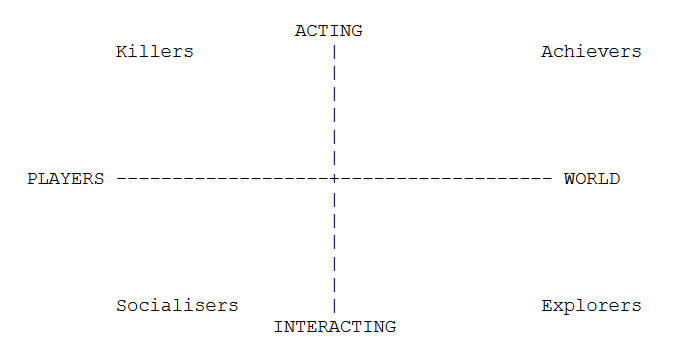
\includegraphics[width=1\linewidth]{content/pictures/basic_interests.PNG}
\caption{Interessen Graph nach Bartle (vgl. \cite{bartle_hearts_1996})}
\label{fig:bartle-muds}
\end{figure}

In X-Achsen-Richtung wird unterschieden, ob der Spieler seine Spielerfahrung über das Verhalten der anderen Mitspieler (Players) oder der Spielwelt (World) bevorzugt. Auf der Y-Achsen-Richtung unterscheidet er, ob der Spieler bevorzugt, selbst einen Einfluss auf die Spielwelt zu geben und diese beeinflusst (Acting) oder ob er in tiefere Interaktion mit der Spielwelt eingehen will (Interacting).

Die daraus resultierenden Typen sind:
\paragraph{Achiever}
Sie sind daran interessiert, auf die Welt einzuwirken, um dadurch in sie eintauchen zu können. Sie wollen das Spiel meistern und dazu bringen, das zu tun, was sie wollen. Ihr Status im Spiel ist ihnen wichtig und die wenige Zeit, die sie dafür benötigt haben.

\paragraph{Explorer}
Sie wollen vom Spiel überrascht werden und mit der Spielwelt interagieren. Die virtuelle Welt löst ein Gefühl des Staunens aus, nach dem sie sich sehnen. Sie sind stolz auf das Wissen über das Spiel, das sie sammeln, und wollen dieses Wissen gerne an neue Spieler weitergeben.

\paragraph{Socialiser}
Sie wollen mit anderen Spielern interagieren. Zumeist erfolgt das über Gespräche, es kann aber auch ungewöhnliche Verhaltensweisen einschließen. Andere Menschen kennenzulernen und mehr über sie zu erfahren, ist für sie wertvoller als für andere. Die Spielwelt ist für sie nur eine Kulisse, für sie sind andere Charaktere fesselnder. Sie sind stolz auf Freundschaften, ihre Kontakte und ihren Einfluss.

\paragraph{Killer}
Sie sind daran interessiert, auf andere Spiele einzuwirken und mit ihnen Dinge zu machen. Im Allgemeinen erfolgt dies ohne das Einverständnis der anderen Spieler. Sie wollen ihre Überlegenheit gegenüber anderen Menschen demonstrieren. Sie sind stolz auf ihren Ruf und oft geübten Kampffähigkeiten.

(vgl. \cite{bartle_hearts_1996}).

\subsection{Erweiterte Einteilungen}
Bartle ist nicht der Einzige, der sich mit Spielertypen auseinandergesetzt hat. Seine Forschung gilt als Fundament, welches in der weiteren Forschung für Diskussionen in der Forschungs- und Game-Design-Community gesorgt hat. 
\begin{quote}
    \textit{
        \enquote{Player types are not a defined concept and any categorization of players or users needs to occur within the context of a particular application or domain. Play-personas are suggested as a useful tool that can be used to put player type research into practice as part of the design process of gamified systems.}
    } 
    (\cite{dixon_player_nodate})
\end{quote}

\paragraph{Dixon} 
stellt Spieler-Personae vor, die wie im \ac{UCD}-Prozess verwendet werden können. Dadurch muss im Designprozess nicht zu sehr zwischen Motivation, Verhalten oder Vorlieben unterschieden werden, da Personae als reichhaltige und erzählerische Darstellung gedacht sind (vgl. \cite{dixon_player_nodate}).

\paragraph{Bateman und Boon}
benutzen in ihrer 2005 erschienen Studie zur Bestimmung des ersten Modells des demografischen Game Designs (DGD1) vier Spielstile, welche sie durch die Hinzunahme der Myers-Briggs Type Indicator (vgl. \cite{noauthor_mbti_nodate}) ableiteten (vgl. \cite{bateman_21st_2005}).
Conquerer (Eroberer), Manager, Wanderer (Wanderer) und Participant (Teilnehmer) waren dabei die vier Spielstile.

In einer zweiten Studie wurden vier hypothetische Spielstile erstellt, welche von einer Studie von Berens 2000 (vgl. \cite{berens_understanding_2000}) abgeleitet wurden (vgl. \cite{bateman_player_2012}). Die resultierenden Stile sind folgende: Logistical, Tactical, Strategic und Diplomatic.

Im Kern sind diese Modelle Ableitungen von Bartles ursprünglicher Metrik (vgl. \cite{ludologie_spielertypen_nodate}).

\paragraph{Yee}
Nick Yee entwickelte empirisch fundiertes Modell zur Beschreibung von Spielmotivationen in Online-Spielen, das bis heute einen großen Einfluss auf die Ludologie hat. Mittels eines faktorenanalytischen Ansatzes untersuchte er eine Vielzahl an Daten aus Online-Umfragen und identifizierte dabei 10 spezifische Motivationsgruppen, die in drei übergeordnete Hauptkategorien gegliedert werden (vgl. \cite{yee_motivations_nodate}):

\begin{figure}[ht]
\centering
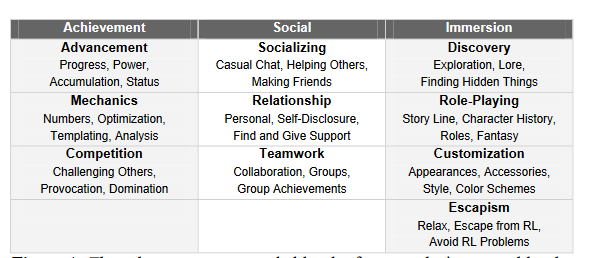
\includegraphics[width=1\linewidth]{content/pictures/nick_yee_categorizations.PNG}
\caption{Motivationsgruppen nach Nick Yee (vgl. \cite{yee_motivations_nodate})}
\label{fig:nick_yee_motivations}
\end{figure}

Die Achievement-Komponente umfasst den Fortschritt im Spiel, sowie das damit einhergehende Verlangen Macht zu erlangen, schnell voranzukommen und Symbole von Reichtum oder Status im Spiel zu erlangen. Außerdem existiert ein Interesse daran, die Mechanik des Spiels zu analysieren, die Regeln und Systeme zu verstehen um die Leistung der Spielfigur zu optimieren. Außerdem ist der Wettbewerb wichtig. Es besteht der Wunsch danach sich mit anderen zu messen und gegen sie anzutreten.

Die soziale Komponente beschreibt dabei die Sozialisierung der Spieler, bei denen sie Interesse daran haben anderen Spielern zu helfen und sich mit ihnen zu Unterhalten. Daraus entstehen Beziehungen, bei denen der Wunsch nahe liegt, dass langfristige und bedeutungsvolle Beziehungen zu anderen aufgebaut werden können. Außerdem ist Teamarbeit gewünscht, um sich gegen andere zu messen und gegen sie anzutreten.

Die Immersions-Komponnete beschreibt das Entdecken in der Spielwelt und dem damit einhergehende finden von Dingen, Wissen zu erlangen, welches den meisten anderen Spielern unbekannt ist. Rollenspiel-Elemente sind dabei besonders wichtig, um den Spielfiguren eine Hintergrundgeschichte zu geben und gemeinsam eine improvisierte Geschichte zu entwickeln. Der Spielavatar sollte auch anpassbar sein, damit der individuelle Geschmack der Spieler in das Spiel einfließen kann. Die Spiel-Welt wird genutzt um von den Problemen der realen-Welt zu entkommen.

% \cite{bartle_hearts_nodate}

% [erwähnen wurde aber rausgelassen, man kann erwähnen, dass es noch weitere klassifizierungen gibt
% \subsection{Das BrainHex-Model}
% \cite{nacke_brainhex_2014}
% ]

% [kommt zu wichtige Begriffe
% \section{Kooperative Gamedesign Pattern}
% \subsection{Was sind Game Pattern}
% \cite{bjork_patterns_2005}

% \subsection{Complementarity}

% \subsection{Synergies}

% \subsection{Abilities}

% \subsection{Shared Goals}

% \subsection{Synergies between goals}

% \subsection{Special Rules for Player of the same Team}

% \subsection{Camera Setting}

% \subsection{Interacting with the same object}

% \subsection{Shared puzzle}

% \subsection{Shared characters}

% \subsection{Special characters targetting lone wolf}

% \subsection{Vocalization}

% \subsection{Limited ressources}

% \subsection{Einflussnahme}
% \cite{emmerich_impact_2017}

% ]
\section{Multiplayerspiele}

\subsection{Klassifizierungen}

\subsubsection{Synchrone Multiplayer}

\subsubsection{Asynchrone Multiplayer}

\subsubsection{Symmetrische Multiplayer}

\subsubsection{Asymmetrische Multiplayer}

\subsection{Artverwandte Beispiele}
Hier kommen die analysierten Spiele rein, also die Auflistung der Spiele, die ich mir im Zuge angesehen habe

\section{Netzwerkinfrastrukturen}

enthält eine Liste von Möglichkeiten auf welcher Grundlage verschiedene Multiplayer Anwendungen gebaut werden können


\chapter{Verwandte Arbeiten}

\cite{harris_asymmetry_2019}
\cite{sajjadi_maze_2014}

hier würden Paper reinkommen die asymmetrische Multiplayer gemacht haben, welche aspekte da mitreinspielen, da kommen dann auch die wichtigen Begriffe dazu mitrein. Auch bereits umgesetzt asymetrische VR Spiele?


Auch Anna Lotz´ Thesis wäre hier relevant


\section{Wichtige Begriffe}

\subsection{Interdependence}
\cite{harris_leveraging_2016}
\cite{depping_cooperation_2017}

\subsection{Degrees of Interdependence}
\cite{beznosyk_effect_2012}

\subsection{Soziale Präsenz}

Vertrauen gibts in dem Kontext auch und wie man dan über Spiele aufbaut

\section{Untersuchungsschwerpunkte}